% begin module trig-substitutions-ex1
\begin{frame}
\begin{example} %[Example 1, p. 504]
\begin{columns}[c]
\column{.4\textwidth}
Evaluate $\int \frac{\sqrt{9-x^2}}{x^2}\diff x$.
\begin{itemize}
\item<2->  Let \alert<handout:0| 3-4,7,14,18>{$x = \uncover<4->{3\sin \theta}$}\uncover<4->{, where \alert<handout:0| 10>{$-\pi /2 \leq \theta \leq \pi / 2$}.}
\item<2->  Then \alert<handout:0| 5-6,13>{$\diff x = \uncover<6->{3\cos \theta\diff \theta}$}\uncover<6->{.}
\end{itemize}
\column{.6\textwidth}
\psset{xunit=1.5cm, yunit=1.5cm}
\begin{pspicture}(-0.15,-0.4)(3.3,1.2)
\psframe*[linecolor=white](-0.1,-0.4)(3.3,1.2)
\psline(0,0)(3, 0)(3,1)(0,0)
\psline(2.9,0)(2.9, 0.1)(3,0.1)
\fcAngle{0}{0.339837}{0.6}{$\theta$}
\uncover<handout:0|18->{
\rput[l](3.1, 0.5){$x$}
\rput[br](1.5, 0.55){$3$}
}
\uncover<handout:0|19->{
\rput[t](1.5, -0.1){$\sqrt{9-x^2} $}
}
%bounding box for pdflatex compilation:
\psline[linecolor=red!1](-0.11, -0.4 )(-0.105, -0.4)
\psline[linecolor=red!1](3.3, 1.21)(3.3, 1.205)
\end{pspicture}
%\ \only<handout:0| -17>{%
%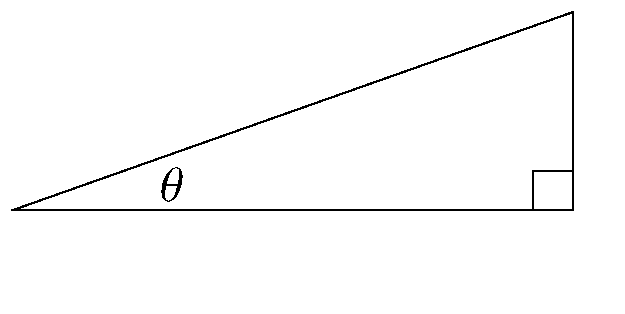
\includegraphics[height=3cm]{trig-substitution/pictures/08-03-ex1a.pdf}%
%}%
%\only<handout:0| 18>{%
%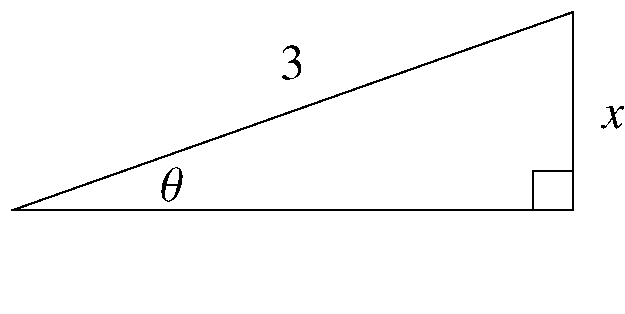
\includegraphics[height=3cm]{trig-substitution/pictures/08-03-ex1b.pdf}%
%}%
%\only<19->{%
%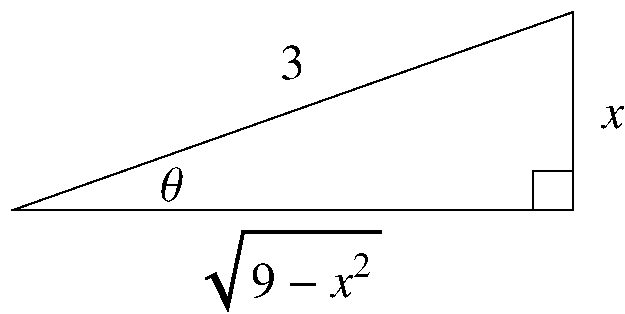
\includegraphics[height=3cm]{trig-substitution/pictures/08-03-ex1c.pdf}%
%}%
\end{columns}
\abovedisplayskip=0pt
\belowdisplayskip=0pt
\[
\uncover<2->{%
\alert<handout:0| 12>{%
\sqrt{9 - \alert<handout:0| 7>{x^2}} =
}%
}%
\uncover<7->{%
\sqrt{9 - \alert<handout:0| 7>{9\sin^2 \theta}} =
}%
\uncover<8->{%
\sqrt{9 \cos^2 \theta} =
}%
\uncover<9->{%
3 |\cos  \theta | =
}%
\uncover<10->{%
\alert<handout:0| 12>{%
3 \cos  \theta
}%
}%
\]
\abovedisplayskip=0pt
\belowdisplayskip=0pt
\begin{eqnarray*}
\uncover<11->{%
\int \frac{\alert<handout:0| 12>{\sqrt{9-x^2}}}{\alert<handout:0| 14>{x^2}}\alert<handout:0| 13>{\diff x}%
}%
& \uncover<11->{ = } & %
\uncover<11->{%
\int\frac{\alert<handout:0| 12>{3\cos \theta}}{\alert<handout:0| 14>{9\sin^2 \theta}}\alert<handout:0| 13>{3\cos \theta \diff \theta}
}%
\uncover<15->{%
 = \int \cot^2 \theta \diff \theta
}\\%
& \uncover<16->{ = } & %
\uncover<16->{%
 \int (\csc^2 \theta  - 1)\diff \theta
}  \uncover<17->{ = }  \uncover<17->{%
 -\alert<handout:0| 20-21>{\cot \theta} - \theta + C
}\\%
& \uncover<21->{ = } & %
\uncover<21->{%
 -\alert<handout:0| 21>{\frac{\sqrt{9-x^2}}{x}} - \Arcsin \left( \frac{x}{3}\right) + C
}%
\end{eqnarray*}
\end{example}
\end{frame}
% end module trig-substitutions-ex1
